\documentclass{standalone}
\usepackage{tikz}

\begin{document}

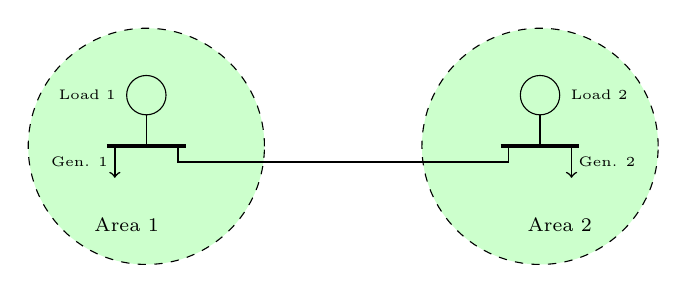
\begin{tikzpicture}
	
	% Area 1
	\draw [dashed, fill=white!80!green] (0.5,0) circle (1.5cm);
		
	% Area 2
	\draw [dashed, fill=white!80!green] (5.5,0) circle (1.5cm);
	
	% Area labels
	\node at (0.25,-1) {\scriptsize Area 1};
	\node at (5.75,-1) {\scriptsize Area 2};
	
	% Bus 1
	\draw [line width=0.5mm] (0,0) -- (1,0);
	\draw [line width=0.2mm] (0.5,0) -- (0.5,0.4);
	
	% Load 1
	\draw [->, line width=0.2mm] (0.1,0) -- (0.1,-0.4);
	\node at (-0.35,-0.2) {\tiny Gen. 1};
	
	% Gen 1
	\draw (0.5,0.65) circle (0.25cm);
	\node at (-0.25,0.65) {\tiny Load 1};
	
	% Bus 2
	\draw [line width=0.5mm] (5,0) -- (6,0);
	\draw [line width=0.2mm] (5.5,0) -- (5.5,0.4);
	
	% Load 2
	\draw [->, line width=0.2mm] (5.9,0) -- (5.9,-0.4);
	\node at (6.35,-0.2) {\tiny Gen. 2};
	
	% Gen 2
	\draw (5.5,0.65) circle (0.25cm);
	\node at (6.25,0.65) {\tiny Load 2};
	
	% Tie line 1 to 2
	\draw [line width=0.2mm] (0.9,0) -- (0.9,-0.2) -- (5.1,-0.2) -- (5.1,0);

\end{tikzpicture}

\end{document}